\documentclass{article}
\usepackage{graphicx,psfrag,epsfig,epsf,latexsym,hhline,amsmath,amssymb,multirow}
\usepackage[usenames,dvipsnames]{pstricks}
\usepackage{pst-plot}
\usepackage{pstricks-add}
\usepackage{color}
\usepackage{stmaryrd}
\usepackage{graphicx}
\usepackage{amsthm}
\usepackage{footnote}
\usepackage{blindtext}
\usepackage{etoolbox}

\usepackage{tikz}
\usepackage{pgfplots}
\usepgflibrary{shapes}
\usetikzlibrary{arrows,shapes,chains,matrix,positioning,scopes,patterns	}
\pgfplotsset{compat=newest}
\pgfplotsset{plot coordinates/math parser=false}

\begin{document}

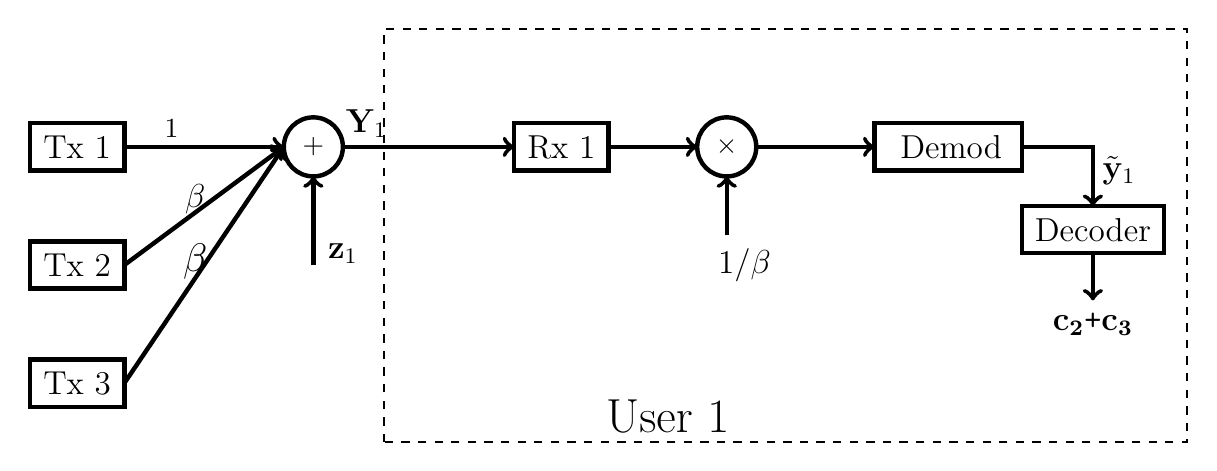
\begin{tikzpicture}[scale=1.5]

%3 Users
\draw[black,ultra thick] (0.4,0.2) rectangle (-0.4,-0.2); \node at (0,0) {\large Tx 1};
\draw[black,ultra thick] (0.4,-0.8) rectangle (-0.4,-1.2); \node at (0,-1) {\large Tx 2};
\draw[black,ultra thick] (0.4,-1.8) rectangle (-0.4,-2.2); \node at (0,-2) {\large Tx 3};

%Oblique lines to Plus block
\draw [->,ultra thick] (0.4,0) -- (1.75,0); \node [above] at (0.8,0) {1};
\draw [->,ultra thick] (0.4,-1) -- (1.75,0); \node [above] at (1,-0.65) {\large $\beta$};
\draw [->,ultra thick] (0.4,-2) -- (1.75,0); \node [above] at (1,-1.2) {\Large $\beta$};


%From + end to Rx1 end
\draw[black,ultra thick] (2,0) circle (0.25); \node at (2,0) {+};
\draw [->,ultra thick] (2,-1) -- (2,-0.25);\node at (2.25,-0.9) {\large $\mathbf{z}_{1}$};

%Receiver 1 block
\draw[black,ultra thick] (3.7,-0.2) rectangle (4.5,0.2); 
\node at (4.1,0) {\large Rx 1};
\draw [->,ultra thick] (2.25,0) -- (3.7,0);
\node[above] at (2.45,0) {\large $\mathbf{Y}_{1}$};

%From Rx1 end to 1/beta multiplicator end
\draw[black,ultra thick] (5.5,0) circle (0.25);
 \node at (5.5,0) {$\times$};
\draw [->,ultra thick] (5.5,-0.75) -- (5.5,-0.25);
\node at (5.65,-1) {\large $1/\beta$};

\draw [->,ultra thick] (4.5,0) -- (5.25,0);

%\draw[black,ultra thick] (4.8,0.4) rectangle (6.2,-0.4); 
%\node[text width=1.2,align=center] at (5.1,0) {\large Subtract $d_{2}\texttt{+}d_{3}$};
%\draw [->,ultra thick] (4.25,0) -- (4.8,0);

% Input to the Demod
\draw[black,ultra thick] (6.75,0.2) rectangle (8,-0.2);
\node at (7.4,0) {\large Demod};
\draw [->,ultra thick] (5.75,0) -- (6.75,0);

%Input to Decoder
\draw [->,ultra thick](8,0) -- (8.6,0) -- (8.6,-0.5);
\node[right] at (8.6,-0.2) {\large $\tilde{\mathbf{y}}_{1}$};
\draw[black,ultra thick] (8,-0.9) rectangle (9.2,-0.5); 
\node at (8.6,-0.7) {\large Decoder};

%Overview dashed rectangle
\draw [->,ultra thick] (8.6,-0.9) -- (8.6,-1.3); 
 \node at (8.6,-1.5){\large $\mathbf{c_{2}}\texttt{+}\mathbf{c_{3}}$};
\draw [dashed,thick] (2.6,-2.5) rectangle (9.4,1);
\node [above] at (5,-2.5) {\LARGE User 1};

 \end{tikzpicture} 
\end{document} 